\documentclass[fleqn,11pt]{article}

\usepackage[letterpaper,margin=0.75in]{geometry}

\usepackage{amsmath}
\usepackage{booktabs}
\usepackage{graphicx}
\usepackage{listings}

\setlength{\parindent}{1.4em}

\begin{document}

\lstset{
  language=Python,
  basicstyle=\small,          % print whole listing small
  keywordstyle=\bfseries,
  identifierstyle=,           % nothing happens
  commentstyle=,              % white comments
  stringstyle=\ttfamily,      % typewriter type for strings
  showstringspaces=false,     % no special string spaces
  numbers=left,
  numberstyle=\tiny,
  numbersep=5pt,
  frame=tb,
}

\title{Network Simulation (Lab 1) Report}

\author{Luke Dickinson}

\date{1/25/2017}

\maketitle

\section{Introduction}

In order to measure the way a basic network performs, we used a network simulator called Bene to simulate a number of different situations. In each of these situations, we will show how the simulation is set up, what the simulation resulted to, and alternate calculations to show that the result from the simulation is correct.

\section{Two Nodes}
This section includes a network that consisting of 2 nodes.


For our first simulation, we set the bandwidth between the nodes to 1 Mbps, and set the propagation delay between the nodes to 1 second. We will send a single packet of size 1000 bytes from one node to the other at time set to 0. To do this we will use the following configuation file:

\begin{lstlisting}
# n1 -- n2
n1 n2
n2 n1

# link configuration
n1 n2 1Mbps 1000ms
n2 n1 1Mbps 1000ms
\end{lstlisting}



Two Nodes: For each of the three scenarios, show the following: (a) your network configuration (similar to the text files in the networks folder), (b) the output of the simulation, and (c) the calculations you used to verify the output is correct.

In order to simulate a simple network of two nodes, we need to create a network configuration file to
Lorem ipsum dolor sit amet, consectetur adipiscing elit. Suspendisse
posuere tellus scelerisque ante luctus eget dapibus ante
egestas. Pellentesque habitant morbi tristique senectus et netus et
malesuada fames ac turpis egestas. Curabitur eget lacus massa, eget
venenatis nisi. Mauris auctor posuere dignissim. Aenean nec tortor
ante, in venenatis arcu. Sed velit turpis, hendrerit ut feugiat
viverra, ultricies tempus nulla. Pellentesque molestie leo ac mi
aliquet sit amet faucibus enim interdum. Phasellus quis sapien
odio. Suspendisse tempor malesuada quam, eget elementum elit placerat
nec. Ut id laoreet risus.

\begin{lstlisting}
class Node:
    def __init__(self,scheduler):
        self.scheduler = scheduler

    def handle_message(self,t,message):
        print "Received at",t,':',message.body
        if message.times < 3:
            self.scheduler.add(t+1.5, message, self.handle_message)
        message.times += 1
\end{lstlisting}

\section{Section Name}

Mauris dictum augue a eros adipiscing mollis. Duis tempus, risus sed
iaculis vehicula, mauris mi aliquam odio, aliquet congue ligula tortor
vitae leo. In convallis, lectus sed egestas tincidunt, augue massa
lacinia augue, a ornare dui magna id enim. Fusce porttitor scelerisque
lorem nec eleifend. Cras lobortis eleifend orci, non lacinia felis
tincidunt eget. Nam vulputate tellus magna, at scelerisque
ligula. Duis dictum bibendum odio nec lobortis. Ut dignissim fringilla
euismod. In pharetra augue et odio blandit malesuada. Nulla lacus
nisi, auctor eget aliquet a, auctor at lorem. Suspendisse nec laoreet
sapien. Nulla facilisi. Nam a congue nunc. Pellentesque auctor turpis
ac augue aliquam convallis. Aenean sit amet eros nibh. Morbi a egestas
libero.

\vspace{0.5cm}
\begin{tabular}{lc}
  \toprule
  Setting & Result\\
  \midrule
  1 & 1.0\\
  2 & 3.45\\
  3 & 7.85\\
  4 & 15.89\\
  \bottomrule
\end{tabular}
\vspace{0.5cm}

Nam sed lacus sit amet nisl bibendum rutrum vel id nisl. Etiam sit
amet ipsum vulputate tellus fringilla tristique a et augue. Etiam
suscipit ante id est lobortis hendrerit. Vivamus vel nisl sit amet
metus volutpat faucibus. Praesent nunc urna, luctus vel convallis
eget, luctus et odio. Nunc et nisl felis. Fusce quis libero sit amet
libero cursus pretium. Vivamus dictum risus non tellus commodo non
bibendum tortor convallis. Cras tempor orci eu leo auctor sed euismod
arcu consectetur. In scelerisque felis et erat commodo
bibendum. Pellentesque hendrerit enim vitae neque sollicitudin
bibendum. In ligula lorem, blandit sit amet aliquet eget, accumsan ut
sem. Maecenas in velit justo. Morbi tellus sem, ultricies in tristique
non, aliquam a lacus. Sed rhoncus blandit ligula, ut eleifend magna
lacinia quis.

\begin{enumerate}

\item Item.

\item Another item.

\end{enumerate}

\section{Section Name}

Donec luctus, libero et egestas tincidunt, arcu ante commodo nunc,
quis sodales leo risus non libero. Mauris ac blandit ligula. Praesent
in dolor non nibh congue blandit. Curabitur in sodales
neque. Curabitur tincidunt nisl nec mauris bibendum
molestie. Suspendisse non justo erat. Ut quis odio elit, sit amet
ullamcorper dui. Nam massa urna, tempus non hendrerit porttitor,
feugiat quis quam. Quisque lacinia cursus nulla, id placerat enim
accumsan et. Donec porta pharetra tincidunt.

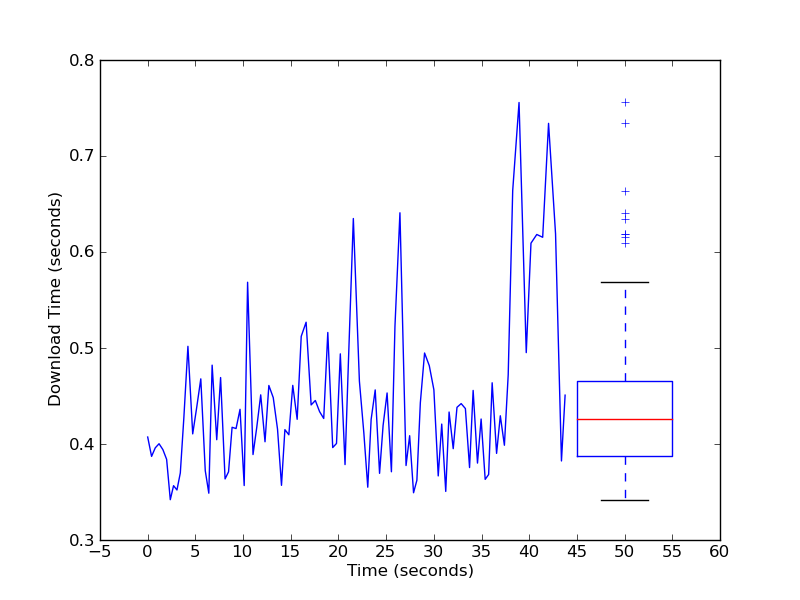
\includegraphics[width=11cm]{graphs/download-combined}

\section{Section Name}

$d_{trans}$ is the transmission delay. $d_{prop}$ is the propagation delay.

\begin{align*}
d &= d_{trans} + d_{prop}\\
  &= (1000*8)/1000000 + 0.05\\
  &= 0.058
\end{align*}

\end{document}
